\documentclass[../../main.tex]{subfiles}
\begin{document}

\begin{flushright}
\footnotesize\textit{【自動文字起こし・要確認】}
\end{flushright}

{\bf [解]}
反射光が半円の中心$O$を中心とする単位円周上を進む様子を考える．$A=(1,0)$から出発し，$k$回目の反射点を$Q_k$とする．円の反射では入射角と反射角（半径となす角）が等しいことから，各反射点の間で弧の中心角は常に一定値$(\pi-2\theta)$ずつ進む．従って
\begin{align}
 \angle Q_1OA = \pi-2\theta,\qquad \angle Q_2OQ_1 = 2(\pi-2\theta)=2\pi-4\theta,\qquad \angle Q_3OQ_2 = 3(\pi-2\theta) \label{eq:1}
\end{align}
である．

% TODO:: 図
\begin{figure}[htb]
\begin{center}
\begin{tikzpicture}[scale=2.2, >=stealth]

  % --- 1. パラメータ設定 (theta = 50度 の例) ---
  \pgfmathsetmacro{\thetaVal}{50}
  
  % 各中心角 (角 AOQ_k)
  % Q1: pi - 2*theta = 80度
  % Q2: 2*(pi - 2*theta) = 160度
  % Q3: 3*(pi - 2*theta) = 240度
  \pgfmathsetmacro{\angQone}{180 - 2*\thetaVal}
  \pgfmathsetmacro{\angQtwo}{2*(180 - 2*\thetaVal)}
  \pgfmathsetmacro{\angQthree}{3*(180 - 2*\thetaVal)}

  % --- 2. 座標軸 ---
  \draw[->, thin, gray] (-1.4,0) -- (1.4,0) node[right, black] {$x$};
  \draw[->, thin, gray] (0,-1.3) -- (0,1.3) node[above, black] {$y$};
  \node[below left, font=\small] at (0,0) {$O$};

  % --- 3. 単位円 ---
  \draw[thick, blue!80!black] (0,0) circle (1);

  % --- 4. 各点の座標 ---
  \coordinate (O) at (0,0);
  \coordinate (A) at (1,0);
  \coordinate (Q1) at ({\angQone}:1);
  \coordinate (Q2) at ({\angQtwo}:1);
  \coordinate (Q3) at ({\angQthree}:1);

  % 交点 P
  \pgfmathsetmacro{\Px}{sin(\thetaVal)/sin(5*\thetaVal)}
  \coordinate (P) at (\Px, 0);

  % --- 5. 光線の軌跡 (A -> Q1 -> Q2 -> Q3) ---
  \draw[ultra thick, red!80!black, ->] (A) -- (Q1);
  \draw[ultra thick, red!80!black, ->] (Q1) -- (Q2);
  \draw[ultra thick, red!80!black, ->] (Q2) -- (Q3);

  % --- 6. 補助線 (半径) ---
  \draw[dashed, gray] (O) -- (Q1);
  \draw[dashed, gray] (O) -- (Q2);
  \draw[dashed, gray] (O) -- (Q3);

  % --- 7. 角度 theta の明記 ---
  
  % (i) 角 OAQ_1 = theta (点 A における内角)
  % 線分 AO (180度方向) から 線分 AQ1 への角
  \draw[->, thin, orange!90!black] ($(A) + (180:0.25)$) arc (180:{180 - \thetaVal}:0.25);
  \node[orange!90!black, font=\scriptsize] at ($(A) + ({180 - \thetaVal/2}:0.35)$) {$\theta$};

  % (ii) 角 AQ_1O = theta (点 Q1 における左側の内角)
  % 線分 Q1A から 線分 Q1O への角
  \draw[->, thin, orange!90!black] ($(Q1) + ({-3*\thetaVal + 360}:0.22)$) arc ({-3*\thetaVal + 360}:{180 + \angQone}:0.22);
  \node[orange!90!black, font=\scriptsize] at ($(Q1) + ({180 + \angQone/2}:0.32)$) {$\theta$};

  % (iii) 角 OQ_1Q_2 = theta (点 Q1 における反射角)
  \draw[->, thin, orange!90!black] ($(Q1) + ({-180 + \angQone}:0.22)$) arc ({-180 + \angQone}:{-180 + \angQone + \thetaVal}:0.22);
  \node[orange!90!black, font=\scriptsize] at ($(Q1) + ({-180 + \angQone + \thetaVal/2}:0.32)$) {$\theta$};

  % --- 8. 中心角 pi - 2*theta ---
  \draw[->, thin, gray] (0.3,0) arc (0:\angQone:0.3);
  \node[gray, font=\scriptsize] at (0.42, 0.22) {$\pi-2\theta$};

  % --- 9. 各点のプロットとラベル ---
  \fill[black] (A) circle (1.2pt) node[below right, font=\small] {$A$};
  \fill[red!80!black] (Q1) circle (1.5pt) node[above right, font=\small] {$Q_1$};
  \fill[red!80!black] (Q2) circle (1.5pt) node[above left, font=\small] {$Q_2$};
  \fill[red!80!black] (Q3) circle (1.5pt) node[below left, font=\small] {$Q_3$};
  \fill[blue!80!black] (P) circle (1.5pt) node[below, font=\small] {$P$};

\end{tikzpicture}
\end{center}
\caption{反射の角度関係（$\angle OAQ_1 = \angle AQ_1O = \theta$）と光の経路}
\end{figure}


\paragraph{(1)}

2回目の反射（$Q_2$）が起こりかつ3回目の反射（$Q_3$）が起こらない条件を求める．
これはすなわち$Q_1,Q_2$が上半円周上にあり，$Q_3$が下半円上にあれば良いから
\begin{align}
 \begin{cases}
  0 < \angle Q_1OA, \angle Q_2OQ_1 < \pi \\
  \pi < \angle Q_3OQ_2 < 2\pi  
 \end{cases}
\end{align}
である．ここに\cref{eq:1}を代入して求める$\theta$の条件は
\begin{align}
 &\begin{cases}
 0 < \pi-2\theta, 2\pi-4\theta < \pi \\
 \pi < 3(\pi-2\theta) < 2\pi  
 \end{cases}
\therefore
 \dfrac{\pi}{4} < \theta < \dfrac{\pi}{3} \label{eq:2}
\end{align}
である．


\paragraph{(2)}

\begin{figure}[htb]
\begin{center}
\begin{tikzpicture}[scale=2.2, >=stealth]

  % --- 1. パラメータ設定 (theta = 50度 の例) ---
  \pgfmathsetmacro{\thetaVal}{55}
  
  % 中心角
  \pgfmathsetmacro{\angQone}{180 - 2*\thetaVal}         % Q1: 80度
  \pgfmathsetmacro{\angQtwo}{2*(180 - 2*\thetaVal)}      % Q2: 160度
  \pgfmathsetmacro{\angQthree}{3*(180 - 2*\thetaVal)}    % Q3: 240度

  % 座標定義
  \coordinate (O) at (0,0);
  \coordinate (A) at (1,0);
  \coordinate (Q1) at ({\angQone}:1);
  \coordinate (Q2) at ({\angQtwo}:1);
  \coordinate (Q3) at ({\angQthree}:1);

  % 点 P の x 座標: sin(theta) / sin(5*theta)
  \pgfmathsetmacro{\Px}{sin(\thetaVal)/sin(5*\thetaVal)}
  \coordinate (P) at (\Px, 0);

  % --- 2. 座標軸 ---
  \draw[->, thin, gray] (-1.4,0) -- (1.4,0) node[right, black] {$x$};
  \draw[->, thin, gray] (0,-1.2) -- (0,1.2) node[above, black] {$y$};
  \node[below right, font=\small] at (O) {$O$};

  % --- 3. 単位円 (薄く表示) ---
  \draw[thick, gray!50] (O) circle (1);

  % --- 4. 【強調】 三角形 Q2OP の色付け ---
  \fill[orange!20] (O) -- (Q2) -- (P) -- cycle;
  \draw[ultra thick, orange!80!black] (O) -- (Q2) -- (P) -- cycle;

  % --- 5. 光線の背景線 (全体像の文脈維持) ---
  \draw[thick, gray!40] (A) -- (Q1) -- (Q2);
  \draw[thick, gray!40] (Q2) -- (Q3);
  \draw[dashed, gray!60] (O) -- (Q2);

  % --- 6. 角度の表示 (triangle Q2OP に必要な角度) ---

  % (i) 角 OQ2P = theta (点 Q2 における内角)
  % 線分 Q2O から 線分 Q2P (Q2Q3) への角
  \draw[->, thick, red!80!black] ($(Q2) + ({3*180 - 5*\thetaVal}:0.22)$) 
    arc ({3*180 - 5*\thetaVal}:{3*180 - 4*\thetaVal}:0.22);
  \node[red!80!black, font=\small] at ($(Q2) + ({3*180 - 4.5*\thetaVal}:0.32)$) {$\theta$};

  % (ii) 角 Q2PO = 2pi - 5theta (点 P における内角)
  % 線分 PO (0度方向) から 線分 PQ2 への角
  \draw[->, thick, red!80!black] ($(P) + (0:0.25)$) arc (0:{180 - (5*\thetaVal - 180)}:0.25);
  \node[red!80!black, font=\scriptsize, above right] at ($(P) + (0.1, 0.05)$) {$2\pi-5\theta$};

  % --- 8. 中心角 pi - 2*theta ---
  \draw[->, thin, gray] (0.3,0) arc (0:{2*\angQone}:0.3);
  \node[gray, font=\scriptsize] at (0.42, 0.22) {$2\pi-4\theta$};

  % --- 7. 辺の長さの表示 ---
  % 半径 OQ2 = 1
  \node[orange!90!black, font=\small, above right] at ($(O)!0.5!(Q2)$) {$1$};

  % --- 8. 各点のプロットとラベル ---
  \fill[black] (A) circle (1.0pt) node[below right, font=\small, gray] {$A$};
  \fill[black] (Q1) circle (1.0pt) node[above right, font=\small, gray] {$Q_1$};
  \fill[red!80!black] (Q2) circle (1.8pt) node[above left, font=\small] {$Q_2$};
  \fill[black] (Q3) circle (1.0pt) node[below left, font=\small, gray] {$Q_3$};
  \fill[red!80!black] (P) circle (1.8pt) node[below, font=\small] {$P$};

\end{tikzpicture}
\end{center}
\caption{正弦定理を適用する $\triangle Q_2OP$ の様子}
\end{figure}

\cref{eq:1}より$\angle Q_2PO=\pi-\angle OQ_2P-\angle AOQ_2 = 2\pi-5\theta$である．そこで三角形$OQ_2P$に正弦定理を用いて
\begin{align}
 & \dfrac{|OP|}{\sin \angle OQ_2P} = \dfrac{|OQ_2|}{\sin \angle OPQ_2} \\
 & \dfrac{|OP|}{\sin\theta} = \dfrac{1}{\sin\left(2\pi-5\theta\right)} \\
\therefore
 |OP| = \dfrac{-\sin\theta}{\sin 5\theta}
\end{align}
である．$P$は負の$x$軸上だから求める座標は
\begin{align}
P=\left(\dfrac{\sin\theta}{\sin5\theta},\ 0\right)
\end{align}
である．

\paragraph{(3)}

$P$の$x$座標を
\begin{align}
 f(\theta)=\dfrac{\sin\theta}{\sin5\theta} \label{eq:3}
\end{align}
とおいてこの動く範囲を求めれば良い．まずは$\sin 5\theta$を$\sin\theta,\cos\theta$で書き直そう．
以下簡単のため $\sin\theta=s,\ \cos\theta=c$ と書く．加法定理，三倍角公式，倍角公式より
\begin{align}
\begin{split}
\sin5\theta
 &=\sin(2\theta+3\theta) \\
 &=\sin2\theta\cos3\theta+\sin3\theta\cos2\theta \\
 &=2sc(4c^3-3c)+(3s-4s^3)(1-2s^2) \\
 &=2s(1-s^2)(1-4s^2)+(3s-4s^3)(1-2s^2) \\
 &=(2s-10s^3+8s^5)+(3s-10s^3+8s^5) \\
 &=5s-20s^3+16s^5 \\
 &=s(16s^4-20s^2+5)
\end{split}
\end{align}
である．

\cref{eq:2}の範囲では$s \neq 0$だから\cref{eq:3}に代入して
\begin{align}
f(\theta)=\dfrac{1}{16s^4-20s^2+5} \label{eq:4}
\end{align}
である．
新しく$t=s^2$とおくと，$\theta\in(\pi/4,\pi/3)$で$s$は単調増加で$t$の範囲は
\begin{align}
 \dfrac{1}{2} < t \dfrac{3}{4} \label{eq:5}
\end{align}
である．\cref{eq:4}で$f(\theta)$を$t$で書き直すと
\begin{align}
f(\theta)=\dfrac{1}{16t^2-20t+5}=\dfrac{1}{16\left(t-\dfrac{5}{8}\right)^2-\dfrac{5}{4}}
\end{align}
である．

\begin{figure}[htb]
\begin{center}
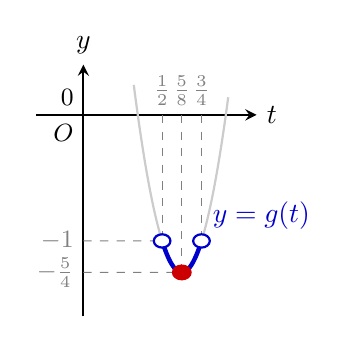
\begin{tikzpicture}[xscale=2, yscale=1.6, >=stealth]

  % --- 1. 座標軸 ---
  \draw[->, thick] (-0.3, 0) -- (1.1, 0) node[right] {$t$};
  \draw[->, thick] (0, -1.6) -- (0, 0.4) node[above] {$y$};
  \node[below left, font=\small] at (0,0) {$O$};

  % --- 2. 注目範囲 1/2 < t < 3/4 の斜線ハッチング ---
  % \begin{scope}
  %   \clip (0.5, -1.6) rectangle (0.75, 0.6);
  %   \fill[pattern=north east lines, pattern color=blue!50]
  %     plot[domain=0.5:0.75, samples=100] (\x, {16*\x*\x - 20*\x + 5})
  %     -- (0.75, -1.6) -- (0.5, -1.6) -- cycle;
  % \end{scope}

  % --- 3. 放物線 y = g(t) 全体（薄線）と 定義域内（太線） ---
  % 全体 (0.3 <= t <= 0.95)
  \draw[thick, gray!40, domain=0.32:0.92, samples=100] 
    plot (\x, {16*\x*\x - 20*\x + 5});

  % 定義域 1/2 < t < 3/4 (太線)
  \draw[ultra thick, blue!80!black, domain=0.5:0.75, samples=100] 
    plot (\x, {16*\x*\x - 20*\x + 5}) node[above right] {$y = g(t)$};

  % --- 4. 頂点（最小値）と端点のプロット・ガイド線 ---
  
  % (i) 頂点 t = 5/8 = 0.625, y = -5/4 = -1.25 (最小値)
  \coordinate (Vertex) at (0.625, -1.25);
  \draw[dashed, gray] (0.625, 0) node[above, font=\small] {$\frac{5}{8}$} -- (Vertex);
  \draw[dashed, gray] (0, -1.25) node[left, font=\small] {$-\frac{5}{4}$} -- (Vertex);
  \fill[red!80!black] (Vertex) circle (1.8pt);
  % \node[red!80!black, font=\small, below] at (Vertex) {最小値 $-\dfrac{5}{4}$};

  % (ii) 左端点 t = 1/2 = 0.5, y = -1 (開区間 -> 白丸)
  \coordinate (LeftEnd) at (0.5, -1.0);
  \draw[dashed, gray] (0.5, 0) node[above, font=\small] {$\frac{1}{2}$} -- (LeftEnd);
  \draw[dashed, gray] (0, -1.0) node[left, font=\small] {$-1$} -- (LeftEnd);
  \draw[blue!80!black, fill=white, thick] (LeftEnd) circle (1.5pt);

  % (iii) 右端点 t = 3/4 = 0.75, y = -1 (開区間 -> 白丸)
  \coordinate (RightEnd) at (0.75, -1.0);
  \draw[dashed, gray] (0.75, 0) node[above, font=\small] {$\frac{3}{4}$} -- (RightEnd);
  \draw[blue!80!black, fill=white, thick] (RightEnd) circle (1.5pt);

  % --- 5. y 軸切片などその他の目盛り ---
  \node[above left, font=\small] at (0, 0) {$0$};

\end{tikzpicture}
\end{center}
\caption{$y = g(t) = 16t^2 - 20t + 5$ のグラフと範囲 $\dfrac{1}{2} < t < \dfrac{3}{4}$ における値域}
\end{figure}

$y=g(t)=16\left(t-\dfrac{5}{8}\right)^2-\dfrac{5}{4}$のグラフから\cref{eq:5}では
\begin{align}
 & g\left(\dfrac{5}{8}\right) \le g(t) < g\left(\dfrac{1^{+}}{2}\right), g\left(\dfrac{3^{-}}{4}\right) \\
 & \dfrac{-5}{4} \le g(t) < -1
\end{align}
だから
\begin{align}
 & \dfrac{1}{-1} < f(\theta) \le \dfrac{1}{-5/4} \\
\therefore
 & -1 < f(\theta) \le \dfrac{-4}{5} 
\end{align}
である．従って$P$の動く範囲は$x$軸上の
 \begin{align}
 -1<x\le-\dfrac{4}{5}
 \end{align}
 （$y=0$）である．図示すると下図太線部（境界は太丸は含んで白丸は含まない）である．

\begin{figure}[htb]
\begin{center}
\begin{tikzpicture}[scale=2.5, >=stealth]

  % --- 1. 座標軸 ($x$ 軸) ---
  \draw[->, thick] (-1.5, 0) -- (0.5, 0) node[right] {$x$};
  \draw[->, thin, gray] (0, -0.3) -- (0, 0.4) node[above, black] {$y$};
  \node[below left, font=\small] at (0,0) {$O$};

  % --- 2. 単位円の原点・参考目盛り ---
  \draw[dashed, gray!50] (-1, -0.2) -- (-1, 0.3);
  \node[below, font=\small] at (-1, 0) {$-1$};

  \draw[dashed, gray!50] (-0.8, -0.2) -- (-0.8, 0.3);
  \node[below, font=\small] at (-0.8, 0) {$-\frac{4}{5}$};

  % --- 3. 点 P の動く領域 (-1 < x <= -4/5) の太線強調 ---
  % 見やすさのため x 軸上に重ねて赤の超太線で描画
  \draw[line width=2.5pt, red!80!black] (-1, 0) -- (-0.8, 0);

  % --- 4. 端点記号 ---
  % x = -1 : 不含み（白丸）
  \draw[red!80!black, fill=white, thick] (-1, 0) circle (1.2pt);

  % x = -4/5 : 含む（黒丸・太丸）
  \fill[red!80!black] (-0.8, 0) circle (1.5pt);

  % --- 5. 領域と点 P のラベル ---
  % 領域を示す矢印とテキスト
  \draw[<-, red!80!black, thick] (-0.9, 0.05) -- (-0.9, 0.25) 
    node[above, red!80!black, font=\small] {$P$ の動く範囲};

\end{tikzpicture}
\end{center}
\caption{点 $P$ の動く範囲（$-1 < x \le -\dfrac{4}{5}, y=0$）}
\end{figure}

\newpage

\end{document}
